\documentclass[xcolor={dvipsnames}, handout]{beamer}
%\documentclass[xcolor={dvipsnames}]{beamer}
\setbeamertemplate{footline}[frame number]
\setbeamersize{description width=-\labelsep}

%\usepackage{amsmath,amsfonts,amssymb,pxfonts,eulervm,xspace}
\usepackage{amsmath, amsfonts, amssymb, mathtools, eulervm, xspace}
\renewcommand{\restriction}{\mathord{\upharpoonright}} %restriction w/p space
\usepackage{relsize} %mathlarger
\usepackage{bm}
\usepackage{centernot}
\usepackage{mathrsfs} % math script fonts
\usepackage{tikz}
\usetikzlibrary{cd} % commutative diagrams
\newtheorem{prop}{Proposition} %math?

\usepackage{subcaption} % subfigure float captioning

\usepackage{tabulary}
\usepackage{tabularx}
%\usepackage{enumitem} $ won't work with beamer
\usepackage{booktabs}
\usepackage{multirow}
\usepackage{array}

\usepackage{graphicx}
\usepackage{adjustbox}%scale tikz-cd

\usepackage{appendixnumberbeamer} 
\usepackage{comment}
\usepackage{minted}
\setminted[python]{fontsize=\scriptsize, 
                   linenos,
                   numbersep=8pt,
                   autogobble, 
                   frame=lines,
                   bgcolor=bg,
                   framesep=3mm} 

\usepackage{notation} % move this later

\graphicspath{.figures/}

\usepackage[backend=bibtex, sorting=none, doi=false,isbn=false,url=false, giveninits=true]{biblatex}
\bibliographystyle{plain}
\bibliography{../paper/bibliography.bib}

%\usetheme{ccnycrest}

\newenvironment{changemargin}[2]{%
\begin{list}{}{%
\setlength{\topsep}{0pt}%
\setlength{\leftmargin}{#1}%
\setlength{\rightmargin}{#2}%
\setlength{\listparindent}{\parindent}%
\setlength{\itemindent}{\parindent}%
\setleng{}th{\parsep}{\parskip}%
}%
\item[]}{\end{list}}

\begin{document}

\title{Topological Equivariant Artist Model}

\begin{frame}<presentation:1|handout:1>
	\titlepage
    Hannah Aizenman, Tom Caswell, Michael Grossberg\\
    %Committee: Dr. Robert Haralick, Dr. Lev Manovich, Dr. Huy Vo\\
    %External Member: Dr. Marcus Hanwell
\end{frame}

\section{Introduction}
\begin{frame}<presentation:1|handout:0>{What are we doing?}
    \begin{itemize}
        \item develop a model for describing data to graphic transformations
        \item specify a visualization library architecture based on this model
        \item implement functional(ish) components based on this model using ideas from functional programming
    \end{itemize}
\end{frame}


%% maybe pull out the middle for now? move the 3 stages down to construction? 
\begin{frame}<presentation:1|handout:0>{What do visualization libraries do?}
    \begin{figure}
        \begin{overprint}
            \onslide<1|handout:1>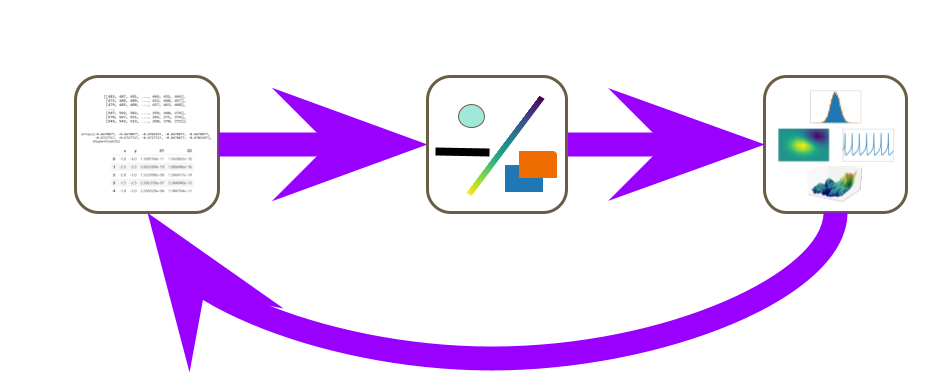
\includegraphics[width=\linewidth]{figures/flow/s2.png}
            \onslide<2|handout:2>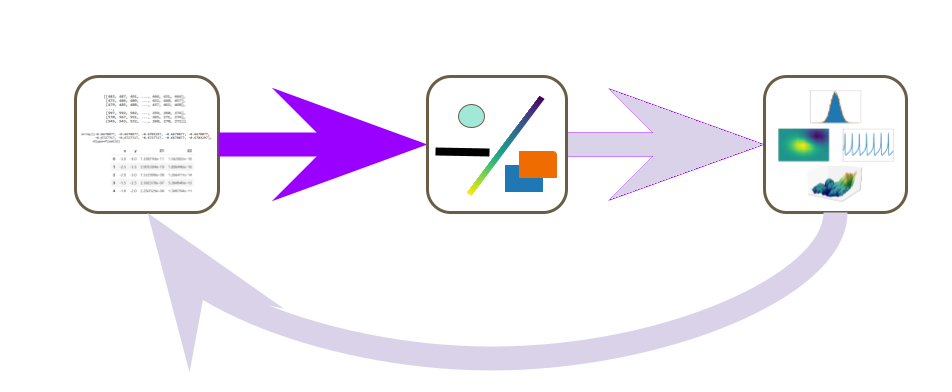
\includegraphics[width=\linewidth]{figures/flow/s_vc.png}
            \onslide<3|handout:3>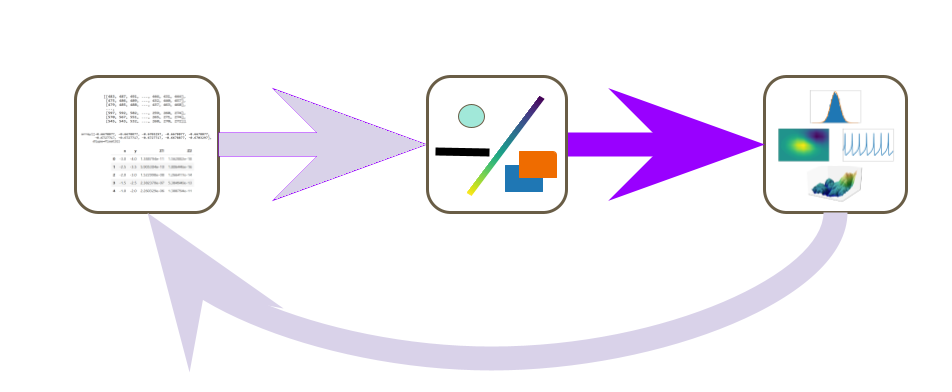
\includegraphics[width=\linewidth]{figures/flow/s_mark.png}
            \onslide<4|handout:4>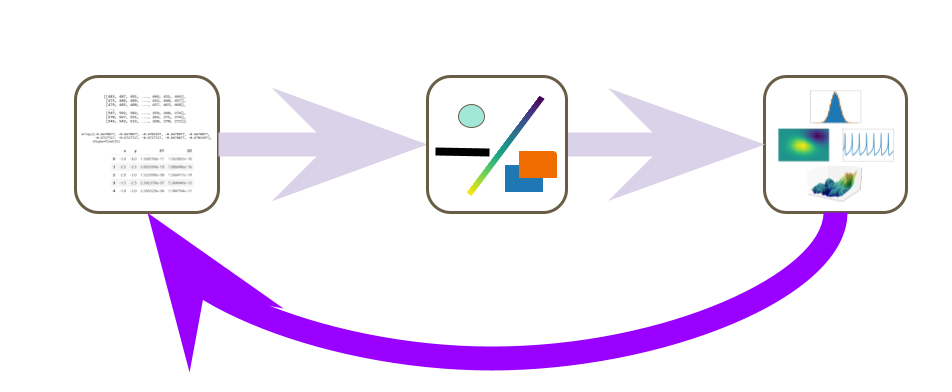
\includegraphics[width=\linewidth]{figures/flow/s3.png}
        \end{overprint}
    \end{figure}
\end{frame}


\begin{frame}<presentation:1|handout:0>{Case Study: Matplotlib}
    \begin{figure}
       
\includegraphics[width=\linewidth]{figures/flow/artists.png}
    \end{figure}
\end{frame}

\begin{frame}<presentation:1|handout:0>{Visualizations Preserve Structure}
    \begin{description}
        \item [continuity] topological properties \cite{wilkinsonGrammarGraphics2005}, i.e. how elements in a dataset are organized, e.g. discrete rows in a table, networked nodes, pixels in an image, points on a line
        \item [equivariance] data and visual encodings are matched such that transformations have an equivalent effect on data and graphical representations, e.g. rotating a matrix and image, shifting  points on a line and a line graphic
      \end{description}
\end{frame}

\begin{frame}<presentation:1|handout:0>{Continuity}
    \begin{figure}
        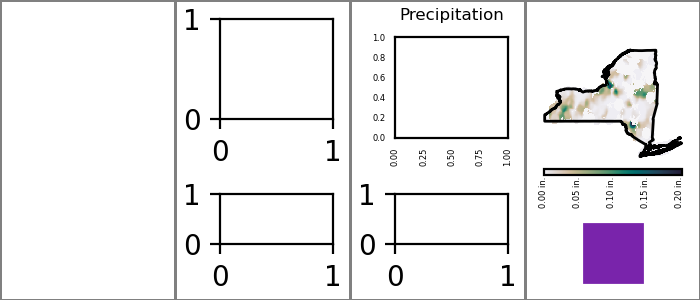
\includegraphics[width=\linewidth]{../paper/figures/k_different_types.png}
    \end{figure}
\end{frame}

\begin{frame}<presentation:1|handout:0>{Expressed in container} 
    \begin{figure}
        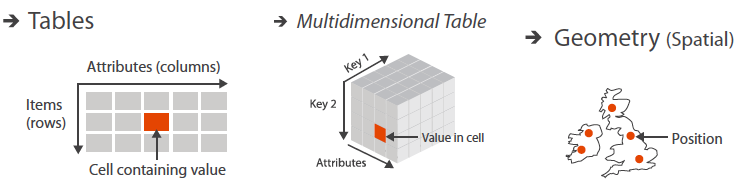
\includegraphics[width=1\textwidth]{figures/intro/munzner_datatypes.png}
        \caption{Figure 2.8 in Munzner's Visualization Analysis and Design\cite{munznerVisualizationAnalysisDesign2014}}
    \end{figure}
\end{frame}

\begin{frame}<presentation:1|handout:0>{Why is container type not enough?}
    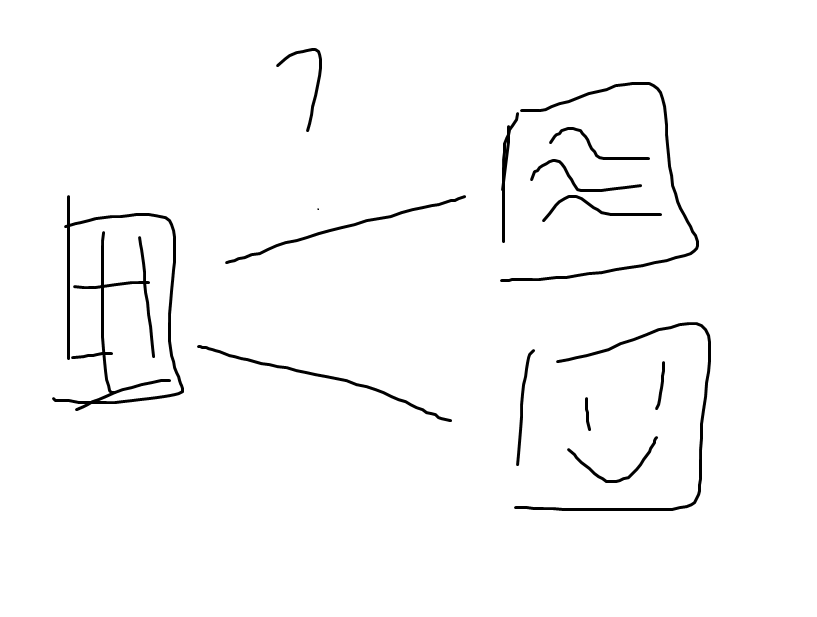
\includegraphics[width=1\linewidth]{../paper/figures/whycontinuity.png}
\end{frame}

\begin{frame}<presentation:1|handout:0>{Equivariance}
    \begin{description}
        \item[Retinal Variables \& Marks] visual encodings should match properties of the data \cite{bertinSemiologyGraphicsDiagrams2011a}
        \pause
        \item[Graphical Integrity] graphs show \textbf{only} the data\cite{tufteVisualDisplayQuantitative2001}
        \pause 
        \item[Naturalness] easier to understand when properties match\cite{norman_things_smart}
        \pause
        \item[Expressiveness] which structure preserving mappings can a tool implement\cite{mackinlayAutomatingDesignGraphical1986}] 
    \end{description}
\end{frame}

%flip columns
\begin{frame}<presentation:1|handout:0>{Frameworks for Expressing Visual Equivariance}
    \begin{description}
        \item[linguistically] visualization has syntax, semantics, grammar expresses how to design structure preserving visualizations
        \cite{mackinlayAutomatingDesignGraphical1986,mackinlayAUTOMATICDESIGNGRAPHICAL1987,wilkinsonGrammarGraphics2005}

        \item[algebraically] transformations on data and graphics are equivalent symmetric \cite{kindlmannAlgebraicProcessVisualization2014}
        \begin{columns}
            \column{.5\textwidth}
            \begin{description}
                \item[D] data 
                \item[R] data representation 
                \item[V] visualization
            \end{description}
            \column{.5\textwidth}
            \begin{equation*}
                \begin{tikzcd}[ampersand replacement=\&]
                    D \arrow[d, "\alpha"'] \arrow[r, "r_1"] \& R \arrow[r, "\nu"]  \& V \arrow[d, "\omega"] \\
                    D \arrow[r, "r_2"']                     \& R \arrow[r, "\nu"'] \& V                    
                \end{tikzcd}
                \end{equation*}
        \end{columns} 
    \item[categorically] \textit{understanding} = \textit{read} $\circ$ \textit{render} \cite{vickersUnderstandingVisualizationFormal2013}    
    \end{description}
\end{frame}

\begin{frame}<presentation:1|handout:0>
    \frametitle{Domain specific libraries know their structure\cite{HeerSoftware2006}}
    \begin{table}
        %\renewcommand{\arraystretch}{2}
        %
        \begin{tabular}{>{\onslide<1->}l>{\onslide<2->}l>{\onslide<3->}l}
            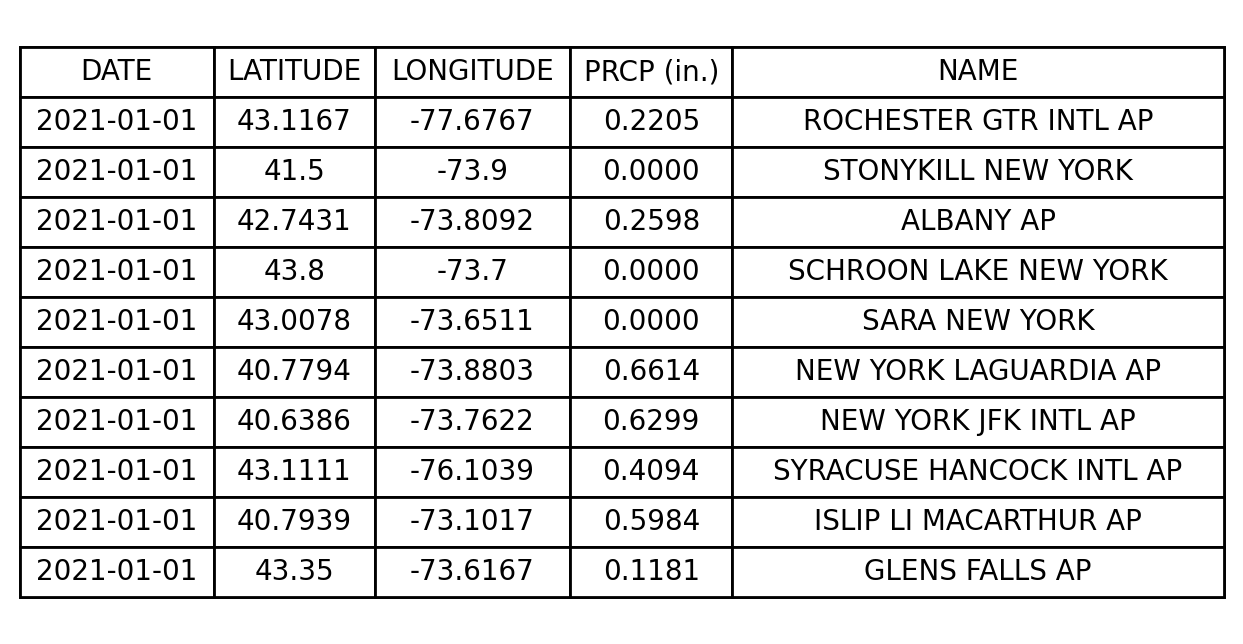
\includegraphics[width=.24\textwidth]{figures/intro/table.png} & 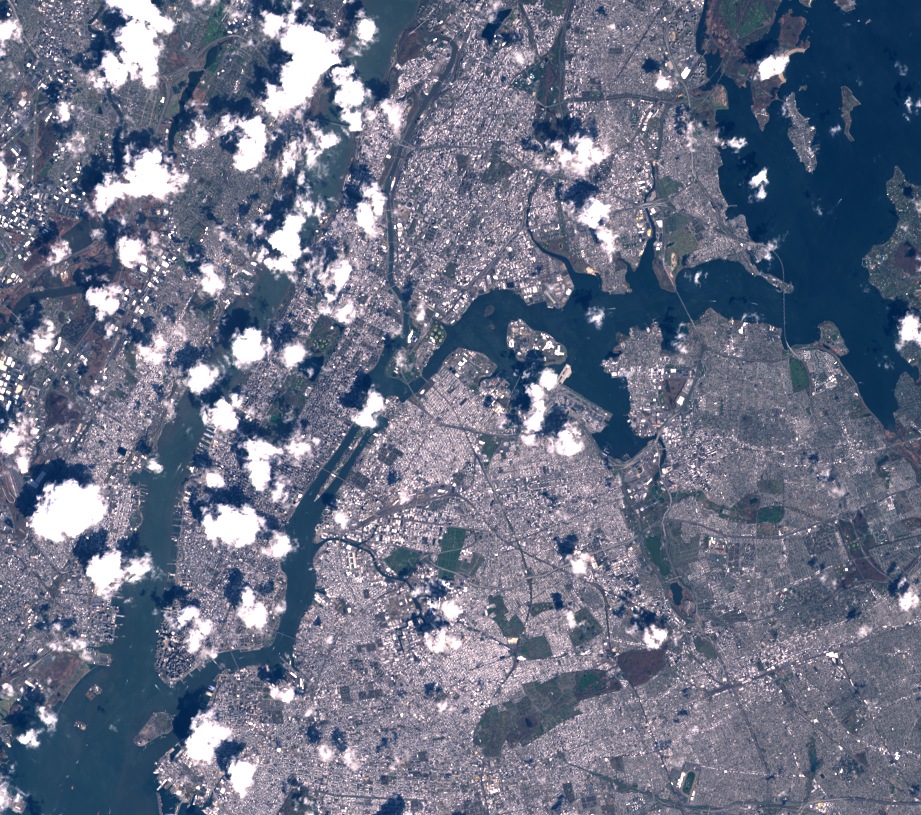
\includegraphics[width=.3\textwidth]{figures/intro/landsat.png} & 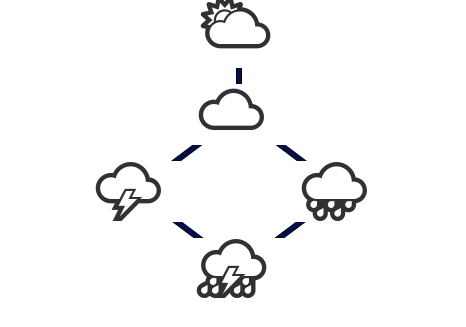
\includegraphics[width=.33\textwidth]{figures/math/graph.png} \\
            ggplot\cite{wickhamGgplot2ElegantGraphics2016a}  & ImageJ\cite{schneiderNIHImageImageJ2012}& Gephi\cite{bastianGephiOpenSource2009}\\
            Vega\cite{satyanarayanDeclarativeInteractionDesign2014} & ImagePlot\cite{studiesCulturevisImageplot2021} & Graphviz\cite{ellsonGraphvizOpenSource2002}\\
            Altair\cite{vanderplasAltairInteractiveStatistical2018}& Napari\cite{nicholas_sofroniew_2021_4533308} & Networkx\cite{HagbergExploringNetwork2008}\\
             Tableau \cite{StoltePolaris2002}& &\\
            \cite{hanrahanVizQL2006,MackinlayShowme2007}&&\\        
        \end{tabular}
    \end{table}
\end{frame}

\begin{frame}<presentation:1|handout:0>
    \frametitle{General purpose libraries generally can't\cite{toryRethinkingVisualizationHighlevel2004}}
    \begin{figure}
        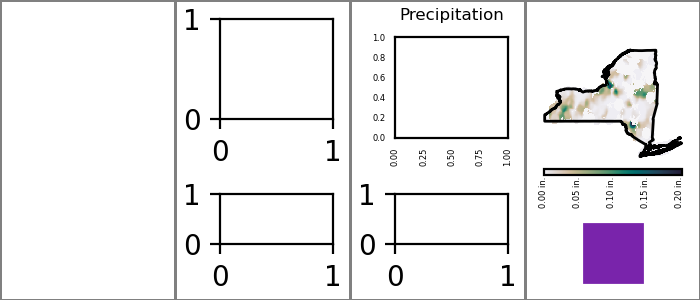
\includegraphics[height=.3\textheight]{../paper/figures/k_different_types.png}
    \end{figure}

    \begin{enumerate}
        \item Matplotlib\cite{hunterMatplotlib2DGraphics2007} $\rightarrow$ Seaborn\cite{waskom2020seaborn}, xarray \cite{hoyer2017xarray} 
        \item D3 \cite{bostockDataDrivenDocuments2011}
        \item VTK \cite{hanwellVisualizationToolkitVTK2015,geveciVTK2012},MayaVi\cite{RamachandranMayaVI2011}$\rightarrow$ Titan\cite{brianwylieUnifiedToolkitInformation2009}, ParaView\cite{ahrens2005paraview}
    \end{enumerate}
\end{frame}

\section{Algebraic Topology & Category Theory}
\begin{frame}<presentation:1|handout:0>{Mathematical Data Abstraction}
    \begin{description}
        \item[Fiber Bundles] "unified, dimension-independent framework" that expresses data as the mapping between continuity and fields \cite{butlerVectorBundleClassesForm1992,butlerVisualizationModelBased1989}
        \item[Category Theory Language] express constraints in specifications \cite{wielsManagementEvolvingSpecifications1998}   
        \item[Sheaves on Bundles] "algebraic data structure" for representing data over topological spaces \cite{ghristElementaryAppliedTopology2014}
    \end{description}
\end{frame}

\subsection{Fiber Bundles}
\begin{frame}<presentation:1|handout:0>
    \frametitle<1|handout:1>{Fiber Bundle}
    \frametitle<6|handout:2-3>{Data Bundle}
    \frametitle<7|handout:4-5>{Graphic Bundle}
    \begin{columns}
        \column{0.31\textwidth}
        \begin{equation*}
            %\label{eq:related-work:continuity:fiber-bundle}
            \begin{tikzcd}[ampersand replacement=\&, row sep=huge]
              \onslide*<3-6|handout:1-2>{\dfiberc}
              \onslide*<7|handout:4>{\gfiberc} 
              \onslide*<4-|handout:1-2,4>{\arrow[r, hook]} \& 
              \onslide*<1-6|handout:1-2>{\dtotalc} 
              \onslide*<7|handout:4>{\gtotalc}
              \onslide*<4-|handout:1-2,4>{\arrow[d, "\pi"']} \\
               \& 
               \onslide*<2-6|handout:1-2>{\dbasec}
               \onslide*<7|handout:4>{\gbasec} 
               \onslide*<5-6|handout:1-2>{\arrow[u, "\dsectionc \in \cgamma{\opensetc}{\dtotalc\restriction_{\opensetc}}"', bend right, pos=.5]}
               \onslide*<7|handout:4>{\arrow[u, "\gsectionc \in \cgamma{\opensetgc}{\gtotalc\restriction_{\opensetgc}}"', bend right, pos=.5]}
            \end{tikzcd}
        \end{equation*}
     \column{0.69\textwidth}
     \only<1-5|handout:1>{
        \begin{description}
            \item<1-5|handout:1>[\textcolor{total}{Total Space}]{$(\dtotalc, \mathcal{T}_{\dtotalc})$}
            \item<2-5|handout:1>[\textcolor{base}{Base Space}]{$(\dbasec, \mathcal{T}_{\dbasec}),\; \dbasepointc \in \opensetc \subseteq \dbasec$}
            \item<3-5|handout:1>[\textcolor{fiber}{Fiber Space}]{$\dfiberc\restriction_{\dbasepointc} = \pi^{-1}(\dbasepointc), \dfiberc = \dfiberc\restriction_{\dbasepointc}\; \forall \dbasepointc \in \dbasec$}
        \end{description}
        }
    \only<6|handout:2>{
        \begin{description}
            \item[\textcolor{total}{Data \dtotalc}]{continuity + fields}
            \item[\textcolor{base}{Continuity \dbasec}]{how data elements are organized (topological properties) \cite{wilkinsonGrammarGraphics2005}, index (key) space \cite{munznerWhatDataAbstraction2014})}
            \item[\textcolor{fiber}{Fields \dfiberc}] {generalization of a schema - named and typed date fields \cite{spivakSIMPLICIALDATABASES, spivakDatabasesAreCategories2010}}
        \end{description}
        }
        \only<7|handout:4>{
            \begin{description}
                \item[\textcolor{total}{Graphic \gtotalc}]{continuity + renderer fields}
                \item[\textcolor{base}{Continuity \gbasec}]{parameterization of graphic area (e.g. "inked" bounding box\cite{CairographicsOrg})}
                \item[\textcolor{fiber}{Display \gfiberc}] {renderer fields, e.g. \{xy,rgba\}, \{xy, cymk\}, \{xyz, rgba\}}
            \end{description}
            }
    \end{columns}
    \pause 
    \only<4-5|handout:1>{
        \begin{alertblock}{}
            \begin{description}
                \item[\textcolor{section}{Sections}]{$\cgamma{\opensetc}{\dtotalc\restriction_{\opensetc}} \coloneqq \big\{\dsectionc: \opensetc\rightarrow \dtotalc\restriction_{\opensetc} \; \bigm{\vert} \pi(\dsectionc(\dbasepointc)) = \dbasepointc\;for\, all\; \dbasepointc \in \opensetc \big\}$}
                \item[Locally Trivial] {for every point $\dbasepointc \in \dbasec$, there exists an open neighborhood $\dbasepointc \in \opensetc \subseteq \dbasec$ s.t. there is a homeomorphism $\pi^{-1}(\opensetc)\xrightarrow{\equivc} \opensetc \times \dfiberc$}
                \item[(Globally) Trivial]{$\dtotalc = \dbasec \times \dfiberc$}
            \end{description}
        \end{alertblock}
    }
    \only<6|handout:2>{
    \begin{alertblock}{}
        \begin{description}
            \item[\textcolor{section}{Data} \cite{butlerVisualizationModelBased1989,butlerVectorBundleClassesForm1992}]{$
        \dsectionc(\dbasepointc) = \;\delementc,\; \dbasepointc\in \opensetc \subseteq \dbasec,\; \delementc \in \dfiberc\restriction_{\dbasepointc}$} 
        \item[]{$\delementc=\{field_0:value, \cdots field_i:value, \cdots field_n:value\}$}
        \end{description}
    \end{alertblock}
    }
    \only<7|handout:4>{
        \begin{alertblock}{}
            \begin{description}
                \item[\textcolor{section}{Graphic}]{$\cgamma{\opensetgc}{\gtotalc\restriction_{\opensetgc}} \coloneqq \big\{\gsectionc: \opensetgc\rightarrow \gtotalc\restriction_{\opensetgc} \; \bigm{\vert} \pi(\gsectionc(\gbasepointc)) = \gbasepointc\;for\, all\; \gbasepointc \in \opensetgc \big\}$}
                \item[] {$\gsectionc(\gbasepointc) = \gelementc,\; \gbasepointc\in \opensetgc\subseteq \gbasec,\; \gelementc \in \dfiberc\restriction_{\gbasepointc}$}
                \item[] $\gelementc=\{x,\,y,\,r,\,g,\,b\}$
           
        \end{description}    
    \end{alertblock}
    }
    \only<|handout:3>{
        \begin{figure}
            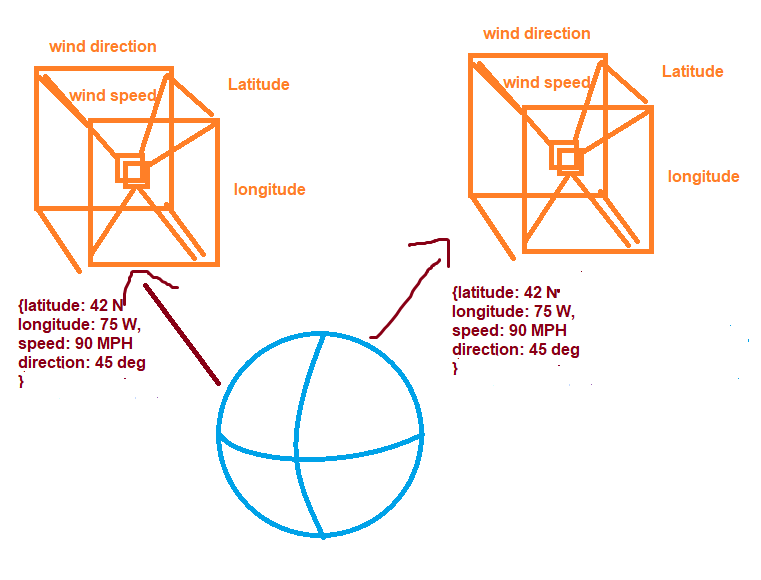
\includegraphics[scale=.65]{figures/math/spherebundle.png}
        \end{figure}
    }
    \only<|handout:5>{
        \begin{figure}
            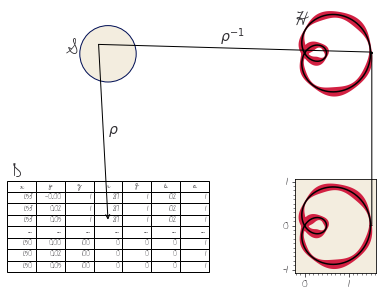
\includegraphics[scale=.65]{figures/math/render.png}
        \end{figure}
    }
\end{frame}

\subsection{Category Theory Language}
\begin{frame}<presentation:1|handout:0>[fragile]{}
    \begin{minted}{python}
        Artist(data:Data) -> Graphic
    \end{minted}
\end{frame}

\begin{frame}<presentation:1|handout:0>{Category $\textcolor{source}{\mathcal{C}}$}
\begin{columns}
    \column{0.39\textwidth}
    \begin{equation*}
    \begin{tikzcd}[ampersand replacement=\&]
        \onslide*<1-|handout:1>{\textcolor{source}{C_1}} 
        \onslide*<3-|handout:1>{\arrow[r, "f", color=source]}
        \onslide*<4-|handout:1>{\arrow[rd, "g\circ f"', color=source]}
        \onslide*<2-|handout:1>{\arrow["id_{C_1}"', loop, distance=2em, in=215, out=145, color=source]} \& 
        \onslide*<1-|handout:1>{\textcolor{source}{C_2}}
        \onslide*<3-|handout:1>{\arrow[d, "g", color=source]} 
        \onslide*<2-|handout:1>{\arrow["id_{C_2}"', loop, distance=2em, in=125, out=55, color=source]} \\\& 
        \onslide*<1-|handout:1>{\textcolor{source}{C_3}}
        \onslide*<2-|handout:1>{\arrow["id_{C_3}"', loop, distance=2em, in=305, out=235, color=source]}              
    \end{tikzcd}
    \end{equation*}
    \column{0.59\textwidth}
    \begin{alertblock}<5-|handout:1>{associativity} 
        if $f: C_1 \rightarrow C_2$, $g: C_2 \rightarrow C_3$ and $h: C_3 \rightarrow C_4$ then $h\circ (g \circ f) = (h \circ g) \circ f$
    \end{alertblock}
    \begin{alertblock}<6-|handout:1>{identity} 
        for every $f: C_1 \rightarrow C_2$ there exists identity morphisms $f \circ id_{C_1} = f = id_{C_2} \circ f$
    \end{alertblock}
    \end{columns}
\end{frame}


\begin{frame}<presentation:1|handout:0>{Opposite Category $\textcolor{source}{\mathcal{C}^{op}}$}
    \begin{columns}
        \column{0.49\textwidth}
    \begin{equation*}
        \begin{tikzcd}[ampersand replacement=\&]
            \textcolor{fade}{C_1} \arrow[r, "f", color=fade] \arrow[rd, "g\circ f"', color=fade] \arrow["id_{C_1}"', loop, distance=2em, in=215, out=145, color=fade] \& \textcolor{fade}{C_2} \arrow[d, "g", color=fade] \arrow["id_{C_2}"', loop, distance=2em, in=125, out=55, color=fade] \\
        \& \textcolor{fade}{C_3} \arrow["id_{C_3}"', loop, distance=2em, in=305, out=235, color=fade]              
        \end{tikzcd}
        \end{equation*}
        \column{0.49\textwidth}
        \begin{equation*}
        \begin{tikzcd}[ampersand replacement = \&]
            \textcolor{source}{C_1} \arrow["id_{C_1}"', loop, distance=2em, in=215, out=145, color=source] \& \textcolor{source}{C_2} \arrow[l, "f"',color=source] \arrow["id_{C_2}"', loop, distance=2em, in=125, out=55, color=source]\\
            \& \textcolor{source}{C_3} \arrow[u, "g"', color=source] \arrow[lu, "f \circ g", color=source] \arrow["id_{C_3}"', loop, distance=2em, in=305, out=235, color=source]
            \end{tikzcd}
        \end{equation*}
        \end{columns}
\end{frame}

\begin{frame}<presentation:1|handout:0>
    \frametitle{Functor $\textcolor{functor}{\bm{F}}: \textcolor{source}{\mathcal{C}} \rightarrow \textcolor{target}{\mathcal{D}}$}
\begin{columns}
    \column{.39\textwidth}
    \begin{equation*}
        \begin{tikzcd}[ampersand replacement = \&, ]
            \onslide*<1-|handout:1>{\textcolor{source}{c}} 
            \onslide*<1-|handout:1>{\arrow[d, "f"', shift right=0, color=source]} 
            \onslide*<3-|handout:1>{\arrow[r, "F", color=functor, maps to]} \& 
            \onslide*<2-3|handout:0>{\textcolor{target}{d}}
            \onslide*<4-|handout:0>{\textcolor{target}{F(c)}} 
            \onslide*<0|handout:1>{\textcolor{target}{F(c)=d}} 
            \onslide*<2|handout:0>{\arrow[d, shift right=0, color=target]}
            \onslide*<3-|handout:0>{\arrow[d, "F(f)", shift right=0, color=target]}
            \onslide*<0|handout:1>{\arrow[d, "F(f)", shift right=3, color=target]} \\
            \onslide*<1-|handout:1>{\textcolor{source}{c^{\prime}}} 
            \onslide*<3-|handout:1>{\arrow[r, "F"', color=functor, maps to]}\& 
            \onslide*<2-3|handout:0>{\textcolor{target}{d^{\prime}}}
            \onslide*<4-|handout:0>{\textcolor{target}{F(c^{\prime})}}
            \onslide*<0|handout:1>{\textcolor{target}{F(c^{\prime})= d^{\prime}}}                    
        \end{tikzcd}
    \end{equation*}
    \column{.59\textwidth}
    \begin{alertblock}<5-|handout:1>{composition}
        \begin{align*}
            \textcolor{functor}{F}(\textcolor{source}{g}) \circ  \textcolor{functor}{F}(\textcolor{source}{f}) = \textcolor{functor}{F} (\textcolor{source}{g}\circ \textcolor{source}{f})
        \end{align*}
    \end{alertblock}
    \begin{alertblock}<6-|handout:1>{identity}
        \begin{align*}
            \textcolor{functor}{F}(\textcolor{source}{id_c}) = \textcolor{target}{id}_{\textcolor{functor}{F}(\textcolor{source}{c})}
        \end{align*}
    \end{alertblock}
\end{columns}
\end{frame}

\subsubsection{Natural Transforms}
\begin{frame}<presentation:1|handout:0>
    \frametitle{Natural Transformation $\textcolor{nattran}{\alpha}: \textcolor{functor}{F} \textcolor{nattran}{\Rightarrow} \textcolor{functor}{G}$}
    \onslide<|handout:1>{
    \adjustbox{scale=3, center}{
        \begin{tikzcd}[ampersand replacement=\&]
            \& {} \arrow[dd, "\alpha" , Rightarrow, shorten=1.5em, color=nattran] \&             \\
          \textcolor{source}{\mathcal{C}} \arrow[rr, "F", bend left, color=functor, maps to] \arrow[rr, "G"', bend right, color=functor, maps to] \& \& \textcolor{target}{\mathcal{D}} \\
            \& {} \&            
          \end{tikzcd}}}
\end{frame}

\begin{frame}<presentation:1|handout:0>
    \frametitle{Natural Transformation $\textcolor{nattran}{\alpha}: \textcolor{functor}{F} \textcolor{nattran}{\Rightarrow} \textcolor{functor}{G}$}
    \begin{equation*}
        \begin{tikzcd}[column sep=huge, ampersand replacement = \&]
            \onslide*<2-|handout:1>{\textcolor{target}{F(c)}}
            \onslide*<2-|handout:1>{\arrow[dd, "F(f)"', color=target]}
            \onslide*<4-5|handout:1>{\arrow[rr, "\alpha_{c}", bend left, color=nattran, Rightarrow]}  
            \onslide*<6|handout:0>{\arrow[rr, "\alpha_{c}", color=nattran, Rightarrow]} \& 
            \onslide*<1-4|handout:1>{\textcolor{source}{c}} 
            \onslide*<1-4|handout:1>{\arrow[dd, "f" description, color=source]}
            \onslide*<3-4|handout:1>{\arrow[r, "G"', color=functor,maps to ]}
            \onslide*<2-4|handout:1>{\arrow[l, "F", color=functor, maps to]} \& 
            \onslide*<3-|handout:1>{\textcolor{target}{G(c)}} 
            \onslide*<3-|handout:1>{\arrow[dd, "G(f)", color=target, maps to]} \\
            {} 
            \onslide*<4|handout:1>{\arrow[rr, dotted, color=nattran, Rightarrow]}
            \onslide*<5|handout:0>{\arrow[rr, color=nattran, Rightarrow]} \& \& {}                      \\
            \onslide*<2-|handout:1>{\textcolor{target}{F(c^{\prime})}} 
            \onslide*<4-5|handout:1>{\arrow[rr, "\alpha_{c^{\prime}}"', bend right, color=nattran, Rightarrow]} 
            \onslide*<4-5|handout:0>{\arrow[rr, "\alpha_{c^{\prime}}"', color=nattran, maps to]}\& 
            \onslide*<1-4|handout:1>{\textcolor{source}{c^{\prime}}}
            \onslide*<2-4|handout:1>{\arrow[l, "F"', color=functor, maps to]} 
            \onslide*<3-4|handout:1>{\arrow[r, "G", color=functor, maps to]} \& 
            \onslide*<3-|handout:1>{\textcolor{target}{G(c^{\prime})}}          
        \end{tikzcd}
    \end{equation*}
\end{frame}

\subsection{Sheaves}

\begin{frame}<presentation:1|handout:0>
    \frametitle{Presheaf: $\sheafc: \mathcal{C}^{op} \textcolor{sheaf}{\rightarrow} \setc $}
    \begin{columns}
    \column{0.29\textwidth}
    \begin{tikzcd}[ampersand replacement=\&, row sep=huge]
        \onslide*<9-|handout:1->{\dfiberc}
        \onslide*<9-|handout:1->{\arrow[r, hook]} \& 
        \onslide*<1-|handout:1->{\dtotalc}
        \onslide*<1-|handout:1->{\arrow[d, "\pi"']} \\
           \& 
        \onslide*<1-|handout:1->{\dbasec}
        \onslide*<3-|handout:1->{\arrow[u, "\dsectionc \in \cgamma{\dbasec}{\dtotalc}"', bend right, pos=.5]}
        \end{tikzcd}
    \column{0.69\textwidth}
        \begin{tikzcd}[ampersand replacement = \&, column sep=small]
            \onslide*<3,6-|handout:0>{{\cgamma{\opensetc_1}{\dtotalc\restriction_{{\opensetc_1}}}}} 
            \onslide*<4-5|handout:0>{{\cgamma{\opensetc_1}{\dtotalc\restriction_{{\opensetc_1}}}}\in \setc}
            \onslide*<0|handout:1>{\setc \ni {\cgamma{\opensetc_1}{\dtotalc\restriction_{{\opensetc_1}}}}}
            \&  
            {} \& 
            \onslide*<6-|handout:1>{{\cgamma{\opensetc_2}{\dtotalc\restriction_{\opensetc_2}}}} 
            \onslide*<7-|handout:1>{\arrow[ll, "\iota^*"', hook', color=set]} \\\& \&\\
            \onslide*<3|handout:0>{\opensetc_1 \subset \dbasec}
            \onslide*<4-5|handout:0>{\opensetc_1 \in Ob(\mathcal{\dbasec}^{\textcolor{base}{op}})}
            \onslide*<6-|handout:0>{\opensetc_1}
            \onslide*<0|handout:1>{Ob(\mathcal{\dbasec}^{\textcolor{base}{op}}) \ni \opensetc_1} 
            \onslide*<5-|handout:0>{\arrow[uu, "\sheafc_{\dbasec, \dtotalc}", maps to, color=sheaf]}
            \onslide*<0|handout:1>{\arrow[uu, "\sheafc_{\dbasec, \dtotalc}", maps to, color=sheaf, shift right = 10]}
            \onslide*<7-|handout:1>{\arrow[rr, "\iota"', hook, color=base]} \&   
            \onslide*<8-|handout:1>{\arrow[uu, "\sheafc_{\dbasec, \dtotalc}" description, maps to, color=sheaf]} \& 
            \onslide*<6-|handout:1>{\opensetc_2} 
            \onslide*<6-|handout:1>{\arrow[uu, "\sheafc_{\dbasec, \dtotalc}"', maps to, color=sheaf]}                   
            \end{tikzcd}
    \end{columns}
    \begin{center}
        \begin{alertblock}<8-|handout:1>{stalk}
            \begin{align*}
                \sheafc_{\dbasec, \dtotalc}\restriction_{\dbasepointc}\coloneqq \lim\limits_{\opensetc\ni \dbasepointc} \Gamma(\opensetc, \dtotalc\restriction_{\opensetc}) \\
                 \dfiberc_{\dbasepointc} \subset  \sheafc_{\dbasec, \dtotalc}\restriction_{\dbasepointc}
            \end{align*}
        \end{alertblock}

        \begin{alertblock}<9-|handout:1>{germ}
            %germ  is tau at limit, \tau(k) \in germ
            \begin{align*}
                \dsectionc(\dbasepointc) \in \sheafc_{\dbasec, \dtotalc}\restriction_{\dbasepointc}
            \end{align*}
        \end{alertblock}
    \end{center}
\end{frame}

\begin{frame}<presentation:1|handout:0>{Sheaves on Bundles}
    A sheaf is a presheaf that satisfies the following two axioms\cite{bakerMathsSheaf}\\
    \begin{block}<2-|handout:1>{locality}
        \onslide<3-|handout:1>{
        given $\opensetc = \bigcup\limits_{i\in I} \opensetc_i$ and $\dsectionc^{a}, \dsectionc^{b} \in \sheafc(\opensetc)$,}
        \onslide<4|handout:1>{\\
        if $\dsectionc^{a}\restriction_{\opensetc_i} = \dsectionc^{b}\restriction_{\opensetc_i}$ for each $\opensetc_i \in \opensetc$}
        \onslide<4|handout:1>{then $\dsectionc^{a} = \dsectionc^{b}$}
    \end{block} 
    \begin{block}<5-|handout:1>{gluing} 
         given $\dsectionc^{i} \in \sheafc(\opensetc_i)$
        \onslide<6-|handout:1>{s.t. ${\dsectionc^{i}}\restriction_{\opensetc_i\cap \opensetc_j} = {\dsectionc^{j}}\restriction_{\opensetc_i \cap \opensetc_j}$ for $\opensetc_i, \opensetc_j \in \opensetc$,}
        \onslide<7-|handout:1>{\\there exists $\dsectionc \in \sheafc(\opensetc)$ such that $\dsectionc\restriction_{\opensetc_i} = {\dsectionc^{i}}$} 
    \end{block}      
\end{frame}

\subsubsection{Pullback and Pushforward}
\begin{frame}<presentation:1|handout:1->{}
    \frametitle<3|handout:3>{Function: $\vindexc: \gbasec \rightarrow \dbasec$}
    \frametitle<1|handout:1>{Data}
    \frametitle<4-6|handout:4>{Pullback: data to region of the visualization} 
    \frametitle<2|handout:2>{Graphic}
    \frametitle<7-|handout:5>{Pushforward: visualization to index of data}
    \begin{equation*}
        \begin{tikzcd}[ampersand replacement=\&, row sep=huge]
            \onslide*<0|handout:2,3,5>{\cgamma{\opensetgc}{\gtotalc\restriction_{\opensetgc}}} 
            \onslide*<0|handout:5>{\arrow[rr, "\textcolor{functor}{\vindexpush}", color=functor]} \& \& 
            \onslide*<0|handout:5>{\cgamma{\opensetc}{\vindexpushc\gtotalc\restriction_{\opensetc}}}  
            \\
            \onslide*<0|handout:2,4->{\opensetgc}
            \onslide*<0|handout:3>{\underbrace{\opensetc\times[0,1]^{m}}_{\opensetgc}}
            \onslide*<0|handout:3->{\arrow[rr, "\vindex", color=functor]}
            \onslide*<0|handout:2,3,5>{\arrow[u, "\sheaf_{\gbasec, \gtotalc}", maps to, color=sheaf]}
            \onslide*<0|handout:4>{\arrow[d, dashed, maps to, "\sheaf_{\gbasec, \vindexpullc\dtotalc}"',color=sheaf]} \&  \& 
            \onslide*<0|handout:1,3->{\opensetc}
            \onslide*<0|handout:1,3-4>{\arrow[d, "\sheaf_{\dbasec, \dtotalc}", maps to, color=sheaf]}
            \onslide*<0|handout:5>{\arrow[u, dashed, maps to, "\sheaf_{\dbasec, \vindexpushc\gtotalc}"', color=sheaf]} \\
            \onslide*<0|handout:4>{\cgamma{\opensetgc}{\vindexpullc\dtotalc\restriction_{\opensetgc}}} 
             \& \& 
            \onslide*<0|handout:1,3-4>{\cgamma{\opensetc}{\dtotalc\restriction_{\opensetc}}}
            \onslide*<0|handout:4>{\arrow[ll, "\textcolor{functor}{\vindexpull}", color=functor]} 
        \end{tikzcd}
    \end{equation*}
    \only<0|handout:1>{% data sheaf
        \begin{itemize}
            \item $\dfiberc \hookrightarrow \dtotalc \xrightarrow{\pi} \dbasec$
            \item $\sheafc_{\dbasec, \dtotalc}:\opensetc \mapsto \cgamma{\opensetc}{\dtotalc\restriction_{\opensetc}}, \opensetc \subset \dbasec$
            \item $\cgamma{\opensetc}{\dtotalc\restriction_{\opensetc}} \ni \dsectionc: \opensetc \rightarrow \dfiberc\restriction_{\opensetc}$
            \item $\dsectionc(\dbasepointc) = \{f_0:v_0, \cdots,\}, \dbasepointc \in \opensetc$
        \end{itemize}
    }
    \only<0|handout:4>{%pulled back data sheaf
        \begin{itemize}
            \item $\vindexpullc\dfiberc \hookrightarrow \vindexpullc\dtotalc \xrightarrow{\pi} \gbasec$
            \item $\vindexpullc\sheafc_{\dbasec,\dtotalc}:\opensetgc \mapsto \cgamma{\opensetgc}{\vindexpullc\dtotalc\restriction_{\opensetgc}}, \opensetgc \subset \gbasec$
            \item $\cgamma{\opensetgc}{\vindexpullc\dtotalc\restriction_{\opensetgc}} \ni \vindexpullc\dsectionc: \opensetgc \rightarrow \vindexpullc\dfiberc\restriction_{\opensetgc}$
            \item $\vindexpullc\dsectionc(\gbasepointc) = \dsectionc(\vindexc(\gbasepointc)) = \dsectionc(\dbasepointc)$
        \end{itemize}
    }
    \only<0|handout:2>{% graphic sheaf
        \begin{itemize}
            \item $\gfiberc \hookrightarrow \gtotalc \xrightarrow{\pi} \gbasec$
            \item $\sheafc_{\gbasec, \gtotalc}:\opensetgc \mapsto \cgamma{\opensetgc}{\dtotalc\restriction_{\opensetgc}}, \opensetgc \subset \gbasec$
            \item $\cgamma{\opensetgc}{\gtotalc\restriction_{\opensetgc}} \ni \gsectionc: \opensetgc \rightarrow \gfiberc\restriction_{\opensetgc}$
            \item $\gsectionc(\gbasepointc) = \{d_0, \cdots\}, \gbasepointc \in \opensetgc$
        \end{itemize}
    }
    \only<0|handout:5>{%pushed forward sheaf
        \begin{itemize}
            \item $\vindexpushc\gfiberc \hookrightarrow \vindexpushc\gtotalc \xrightarrow{\pi} \dbasec$
            \item $\vindexpushc\sheafc_{\gbasec, \gtotalc}:\opensetc \mapsto \cgamma{\opensetc}{\vindexpushc\gtotalc\restriction_{\opensetc}}, \opensetc \subset \dbasec$
            \item $\cgamma{\opensetc}{\vindexpushc\gtotalc\restriction_{\opensetc}} \ni \vindexpushc\gsectionc: \opensetc \rightarrow \vindexpushc \gfiberc\restriction_{\opensetc}$
            \item $\vindexpushc\gsectionc(\dbasepointc) = \gsectionc\restriction_{\vindexpre(\dbasepointc)} = \gsectionc(\gbasepointc)\;\forall \gbasepointc \in \vindexpre(\dbasepointc)$ 
        \end{itemize}
    }
\end{frame}

\begin{frame}<presentation:1|handout:0>{Example: Scatter Plot}
    \begin{figure}
        \includegraphics[scale=.1]{figures/math/push_pull_scatter.png}
    \end{figure}
\end{frame}

\begin{frame}<presentation:1|handout:0>{Example: Line Plot}
    \begin{figure}
        \includegraphics[scale=.1]{figures/math/push_pull_line.png}
    \end{figure}
\end{frame}

\begin{frame}<presentation:1|handout:0>{Example: Image}
    \begin{figure}
        \includegraphics[scale=.1]{figures/math/push_pull_image.png}
    \end{figure}
\end{frame}

\begin{frame}<presentation:1|handout:0>{Example: Heatmap}
    \begin{figure}
        \includegraphics[scale=.1]{figures/math/push_pull_heat.png}
    \end{figure}
\end{frame}

\begin{frame}<presentation:1|handout:0>{Example: Sphere}
    \begin{figure}
        \includegraphics[scale=.1]{figures/math/push_pull_sphere.png}
    \end{figure}
\end{frame}

%add transition slide->possibly call back 

\section{Artist}

\begin{frame}<presentation:1|handout:0>
    \frametitle<0|handout:1>{Artist: $\vartistc: \sheafc_{\dbasec, \dtotalc} \rightarrow \sheafc_{\gbasec, \gtotalc}$}
    \frametitle<0|handout:2>{Data Space: $\vartistc_{\opensetc}: \sheafc_{\dbasec, \dtotalc} \textcolor{artist}{\Rightarrow} \vindexpushc\sheafc_{\gbasec, \gtotalc}$}
    \frametitle<0|handout:3>{Display Space: $\vartist_{\opensetgc}: \vindexpullc\sheafc_{\dbasec, \dtotalc} \textcolor{artist}{\Rightarrow} \sheafc_{\gbasec, \gtotalc}$}
    \frametitle<0|handout:4>{Artist: $\vartistc: \cgamma{\opensetc}{\dtotalc} \rightarrow \cgamma{\opensetgc}{\gtotalc}$}
    \onslide*<0|handout:1,4>{
    \begin{equation*}
        \begin{tikzcd}[ampersand replacement=\&]
          \onslide*<0|handout:1>{\sheafc_{\gbasec, \gtotalc}} 
          \onslide*<0|handout:4>{\cgamma{\opensetgc}{\gtotalc\restriction_{\opensetgc}}}
          \onslide*<0|handout:1,4>{\arrow[rr, "\textcolor{functor}{\vindexpush}", color=functor]}  
          \& \& 
          \onslide*<0|handout:1>{\vindexpushc\sheafc_{\gbasec, \gtotalc}}
          \onslide*<0|handout:4>{\cgamma{\opensetc}{\vindexpushc \gtotalc\restriction_{\opensetc}}}
          \\
          \& \& \\
          \onslide*<0|handout:1>{\textcolor{functor}{\vindexpull}\sheafc_{\dbasec, \dtotalc}}
          \onslide*<0|handout:4>{\cgamma{\opensetgc}{\vindexpullc \dtotalc\restriction_{\opensetgc}}}
          \onslide*<0|handout:1,4>{\arrow[uu, "\vartistc_{\opensetgc}", color=artist, Rightarrow]}
          \&  \& 
          \onslide*<0|handout:1>{\sheafc_{\dbasec, \dtotalc}}
          \onslide*<0|handout:4>{\cgamma{\opensetc}{\dtotalc\restriction_{\opensetc}}}
          \onslide*<0|handout:1,4>{\arrow[ll, "\textcolor{functor}{\vindexpull}", color=functor]} 
          \onslide*<0|handout:1,4>{\arrow[uu, "\vartistc_{\opensetc}"', color=artist, Rightarrow]}
          \onslide*<4-|handout:1,4>{\arrow[lluu, "\vartistc"' description, dashed, color=artist, Rightarrow]}
        \end{tikzcd}
    \end{equation*}}
    
    \onslide*<1|handout:2>{
        \begin{equation*}
      \begin{tikzcd}[ampersand replacement =\&]
        \cgamma{\opensetc_1}{\dtotalc} 
        \arrow[dd, "\iota^*"', hook, color=set] 
        \arrow[rrrr, "\vartistc_{\opensetc_1}", bend left, color=artist, Rightarrow] \&  \& 
        \opensetc_1 
        \arrow[ll, "\sheafc_{\dbasec,\dtotalc}", color=sheaf, maps to] 
        \arrow[rr, "\sheafc_{\dbasec,\gtotalpushc}"', color=sheaf, maps to] \&  \& 
        \cgamma{\opensetc_1}{\gtotalpushc} 
        \arrow[dd, "\iota^*", hook', color=set] \\
        {} 
        \arrow[rrrr, dotted, color=artist,Rightarrow] \&\&\&\& {} \\
        \cgamma{\opensetc_2}{\dtotalc} 
        \arrow[rrrr, "\vartistc_{\opensetc_2}"', bend right, color=artist, Rightarrow] \&  \& 
        \opensetc_2 
        \arrow[ll, "\sheafc_{\dbasec,\dtotalc}"', color=sheaf, maps to] 
        \arrow[rr, "\sheafc_{\dbasec,\gtotalpushc}", color=sheaf, maps to] 
        \arrow[uu, "\iota" description, hook, color=base] \& \& 
        \cgamma{\opensetc_2}{\gtotalpushc}               
    \end{tikzcd}
        \end{equation*}}

    \onslide*<0|handout:3>{
        \begin{equation*}
    \begin{tikzcd}[ampersand replacement =\&]
    \cgamma{\opensetgc_1}{\dtotalpullc\restriction_{\opensetgc_1}} 
    \arrow[dd, "\iota^*"', hook, color=set] 
    \arrow[rrrr, "\vartistc_{\opensetgc_1}", bend left, color=artist, Rightarrow] \&  \& 
    \opensetgc_1 
    \arrow[ll, "\sheafc_{\gbasec, \dtotalpullc}", color=sheaf, maps to] 
    \arrow[rr, "\sheafc_{\gbasec,\gtotalc}"', color=sheaf, maps to] \&  \& 
    \cgamma{\opensetgc_1}{\gtotalc\restriction_{\opensetgc_1}} 
    \arrow[dd, "\iota^*", hook', color=set] \\
    {} 
    \arrow[rrrr, dotted, color=artist, Rightarrow] \&\&\&\& {} \\
    \cgamma{\opensetgc_2}{\dtotalpullc\restriction_{\opensetgc_2}} 
    \arrow[rrrr, "\vartistc_{\opensetgc_2}"', bend right, color=artist, Rightarrow] \&  \& 
    \opensetgc_2 
    \arrow[ll, "\sheafc_{\gbasec,\dtotalpullc}"', color=sheaf, maps to] 
    \arrow[rr, "\sheafc_{\gbasec, \gtotalc}", color=sheaf, maps to] 
    \arrow[uu, "\iota" description, hook, color=base] \& \& 
    \cgamma{\opensetgc_2}{\gtotalc\restriction_{\opensetgc_2}}   
    \end{tikzcd}
        \end{equation*}}    
    \onslide<0|handout:1>{
        \begin{equation*}
        \textcolor{nattran}{Nat}_{\opensetgc}(\textcolor{functor}{\vindexpull}\sheafc_{\dbasec, \dtotalc}, \sheafc_{\gbasec, \gtotalc}) = 
    \textcolor{nattran}{Nat}_{\opensetc}(\sheafc_{\dbasec, \dtotalc}, \textcolor{functor}{\vindexpush}\sheafc_{\gbasec, \gtotalc})
        \end{equation*}
    }
    \onslide<0|handout:4>{
        \begin{alertblock}{pull data section \dsectionc\ over graphic space $\gbasepointc \in \gbasec$}
            \begin{equation*}
                \vindexpullc\dsectionc(\gbasepointc) = \dsectionc(\vindexc(\gbasepointc)) = \dsectionc(\dbasepointc)
            \end{equation*}
        \end{alertblock}
        \begin{alertblock}{push graphic \gsectionc\ section over data space $\dbasepointc \in \dbasec$}
            \begin{equation*}
                \vindexpushc\gsectionc(\dbasepointc) = \gsectionc\restriction_{\vindexprec(\dbasepointc)} = \gsectionc(\gbasepointc) \forall \gbasepointc \in \vindexprec(\dbasepointc)
            \end{equation*}
        \end{alertblock}
        }
\end{frame}


\subsection{Equivariance}

\begin{frame}<presentation:1|handout:1>{Transform Data}
    \begin{block}{Fiber Bundle Category}
        \begin{description}[style=newline]
            \item[object] $\dfiberc \hookrightarrow \dtotalc \xrightarrow{\pi} \dbasec$
            \item[morphisms] $\dfuncc: \dtotalc \rightarrow \dtotalc^{\prime}$
        \end{description}
    \end{block}
    \begin{block}{Fiber Category}
        The fiber $\dfiberc$ is a  monoidal category (single object w/ bicartesian product operator on category) of an arbitrary type $\mathcal{C}$. The morphisms on the fiber are $Hom(\dfiberc, \dfiberc)$
    \end{block}

    \begin{block}{Data Transformations}
    $\dfuncc:\dtotalc\restriction_{\dbasepointc} \rightarrow \dtotalc^{\prime}\restriction_{\dbasepointc^{\prime}} \in Hom(\dfiberc\restriction_{\dbasepointc},\dfiberc^{\prime}\restriction_{\dbasepointc^{\prime}})$ 
    \end{block} 
\end{frame}

\begin{frame}<presentation:1|handout:1>{$\dfuncc = (\dfunchc, \dfunctc)$}
    \begin{tikzcd}[ampersand replacement = \&]
        \cgamma{\opensetc}{\dtotalc\restriction_{\opensetc}} 
        \arrow[rr, "\dfuncpullc", color=action] 
        \&  \& 
        \cgamma{\opensetc^{\prime}}{\dfuncpullc\dtotalc\restriction_{\opensetc^{\prime}}} 
        \arrow[rr, "\dfunctc", color=action] 
        \&  \& 
        \cgamma{\opensetc^{\prime}}{\dtotalc^{\prime}\restriction_{\opensetc^{\prime}}} \\
        \&  \&  
        \&  \& \\
        \opensetc 
        \arrow[uu, "{\sheafc_{\dbasec, \dtotalc}}", maps to, color=sheaf]                 
        \&  \& 
        \opensetc^{\prime} 
        \arrow[ll, "\dfunchc", color=action] 
        \arrow[uu, "{\sheafc_{\dbasec^{\prime}, \dfuncpullc\dtotalc}}"', maps to, color=sheaf] 
        \arrow[rruu, "{\sheafc_{\dbasec^{\prime}, \dtotalc^{\prime}}}"', maps to, color=sheaf] 
        \&  \& 
    \end{tikzcd}
    \begin{itemize}
        \item Base Transformation: $\dfunchc: \opensetc^{\prime} \rightarrow \opensetc$
        \item Fiber Transformation: $\dfunctc: \dfuncpullc \dtotalc \rightarrow \dtotalc^{\prime}$ s.t. $\pi(\dfuncpullc\dtotalc) = \pi(\dtotalc^{\prime})$ 
        \item Section Transform: $\dfuncc: \dsectionc\restriction_{\opensetc} \mapsto \dsectionc^{\prime}\restriction_{\opensetc^{\prime}}$
    \end{itemize}
\end{frame}


\begin{frame}<presentation:1|handout:1>{Equivariant Artist}
    \begin{equation*}
        \begin{tikzcd}[ampersand replacement=\&]
            \sheafc_{\dbasec, \dtotalc} 
            \arrow[r, "\vartistc", Rightarrow, color=artist] 
            \arrow[d, "\dfuncc_{\dtotalc}"', color=action] \& 
            \sheafc_{\gbasec, \gtotalc} 
            \arrow[d, "\dfuncc_{\gtotalc}", color=action, dashed] \\
            \sheafc_{\dbasec^{\prime}, \dfuncpullc\dtotalc} 
            \arrow[r, "\vartistc", Rightarrow, color=artist]\& 
            \sheafc_{\gbasec^{\prime},\dfuncpullc\gtotalc}
        \end{tikzcd} 
        \end{equation*}

    \begin{alertblock}{Artist Constraints}
        \begin{align*}
            \vartistc(\dsectionc^{a}) = \vartistc(\dsectionc^{b}) &\centernot\implies \dsectionc^a = \dsectionc^b \\
            \vartistc(\dsectionc^{a})  = \vartistc(\dsectionc^{b}) &\implies \vartistc(\dfuncc_{\dtotalc}(\dsectionc^{a})) = \vartistc(\dfuncc_{\dtotalc}(\dsectionc^{b}))
        \end{align*}
    \end{alertblock}
\end{frame}

\begin{frame}<presentation:1|handout:1>{Equivariant $\dfunchc$}
    \note{Maybe move to implementation section}
        \begin{equation*}
            \begin{tikzcd}[ampersand replacement=\&]
            \opensetgc 
            \arrow[rr, "\vindexc", color=functor] 
            \arrow[dd, "\dfunchc_{\gbasec}"', dashed, color=action] 
            \&  \& 
            \opensetc 
            \arrow[dd, "\dfunchc_{\dbasec}", color=action] \\
            \&  \& \\
            \opensetgc^{\prime} 
            \arrow[rr, "\vindexc"', color=functor]
            \&  \& 
            \opensetc^{\prime}\\
            \underbrace{\dbasec \times {[0,1]}^{m}}_{\gbasec} \arrow[rr,"\vindex", maps to, color=functor] \& \& \dbasec
            \end{tikzcd}
        \end{equation*}
\end{frame}

\begin{frame}<presentation:1|handout:1>{Checking if \vartistc\ is equivariant}
    \begin{equation*}
        \begin{tikzcd}[ampersand replacement=\&, row sep=huge]
            \cgamma{\opensetc}{\dtotalc\restriction_{\opensetc}} 
            \arrow[rr, "\vartistc", Rightarrow, color=artist] \&  \& 
            \cgamma{\opensetgc}{\gtotalc\restriction_{\opensetgc}} 
            \arrow[rrd, "\delta"'] 
            \arrow[rr, "render"] \&  \& visualization 
            \arrow[d, "measure" description] \\ 
            \&  \&  \&  \& M
            \end{tikzcd}
    \end{equation*}
    \begin{alertblock}{Visual Measurement $\delta$}
        \begin{equation}
            \delta: \cgamma{\opensetgc}{\gtotalc\restriction_{\opensetgc}} \rightarrow M
        \end{equation}
        $M$ is a measurable component of the rendered visual element, e.g. color, position, shape, texture
    \end{alertblock}
\end{frame}


\begin{frame}<presentation:1|handout:1>{Checking if \vartistc\ is equivariant}
    \begin{equation*}
        \begin{tikzcd}[ampersand replacement=\&]
            \cgamma{\opensetc}{\dtotalc\restriction_{\opensetc}} 
            \arrow[rr, "\vartistc"', Rightarrow, color=artist] 
            \arrow[d, "\dfuncc_{\dtotalc}"', color=action] 
            \arrow[rrr, "\equivc", bend left, color=monoid, dashed] \&  \& 
            \cgamma{\opensetgc}{\gtotalc\restriction_{\opensetgc}} 
            \arrow[r, "\delta"']\& M 
            \arrow[d, "\dfuncc_{M}", color=action] \\
            \cgamma{\opensetc^{\prime}}{\dfuncpullc\dtotalc\restriction_{\opensetc^{\prime}}} 
            \arrow[rr, "\vartistc", Rightarrow, color=artist] 
            \arrow[rrr, "\equivc"', bend right, color=monoid, dashed] \&  \& 
            \cgamma{\opensetgc^{\prime}}{\dfuncpullc\gtotalc\restriction_{\opensetgc^{\prime}}} 
            \arrow[r, "\delta"] \& M^{\prime}                        
        \end{tikzcd}
    \end{equation*}
        there exists a functor $\equivc: \dfuncc_{\dtotalc} \rightarrow \dfuncc_{M}$ such that 
        \begin{description}
            \item[equivariance] $\equivc(\dfuncc_{\dtotalc}(\dsectionc(\dbasepointc))) = \dfuncc_{M}(\equivc(\dsectionc(\dbasepointc)))$, for all $\dbasepointc \in \dbasec$ 
            \item[continuity] $\lim\limits_{x\to \dbasepointc}(\equivc(\dsectionc(x))) = \equivc(\dsectionc(\dbasepointc))$ for all $\dbasepointc \in \dbasec$ 
        \end{description} 
\end{frame}

\begin{frame}<presentation:1|handout:0>{Multiple Bundles: $\dfuncc = (\dfunchc, \prod\limits_{i=0}^{n}\dfunctc_i)$}
    \begin{equation*}
        \begin{tikzcd}[ampersand replacement = \&, column sep=2ex]
                \dfunctc_0 \dfuncpullc \dtotalc_0 
                \arrow[rdd, "\pi" description] 
                \arrow[r, "\cdots \otimes \cdots", phantom] \& 
                \dfunctc_i  \dfuncpullc \dtotalc_i 
                \arrow[dd, "\pi" description] 
                \arrow[r, "\cdots \otimes \cdots", phantom] \& 
                \dfunctc_n \dfuncpullc \dtotalc_n 
                \arrow[ldd, "\pi" description] \& = \& 
                \prod\limits_{i=0}^{n} 
                \dfunctc_i \dfuncpullc \dtotalc 
                \arrow[dd, "\pi" description] \\    
                \&\&\&\&\\    
                \& 
                {(\dfunchc=\dfunchc_{i \in [0,n]})\dbasec }                                             \& \& = \& 
                \dfunchc \dbasec                                                        
                \end{tikzcd}                                              
    \end{equation*}

\end{frame}

\begin{frame}<presentation:1|handout:0>{Complex data}
    \begin{description}[style=newline]
        \item[combining continuities]{given $\dbasepointc_{a} \in \dbasec_{c} \subset \dbasec_{a}$ and $\dbasepointc_{b} \in \dbasec_{c} \subset \dbasec_{b}$, if $\dbasepointc_{a} = \dbasepointc_{b}$ then $\equivc(\dsectionc(\dbasepointc_{a})) = \equivc(\dsectionc(\dbasepointc_{b}))$ for all $\dbasepointc_{a}, \dbasepointc_{b} \in \dbasec_{a}\bigsqcup\limits_{\dbasec_{c}} \dbasec_{b}$}
        \item[shared fibers]{
            if $p = p^{\prime}$ then $\equivc \circ q$ = $\equivc^{\prime} \circ q^{\prime}$
        \begin{equation*}
        \begin{tikzcd}[ampersand replacement = \&]
        \& \dfiberc^a \times \dfiberc^b 
        \arrow[ld, "p"', color=fiber] 
        \arrow[rd, "q \circ \equivc"] \&     \\
        \dfiberc^a \& \& M^a \\
        \& \dfiberc^a \times \dfiberc^c 
        \arrow[lu, "p^{\prime}", color=fiber] 
        \arrow[ru, " q^{\prime} \circ\equivc^{\prime}"'] \&    
      \end{tikzcd}
    \end{equation*}}         
        \item[both]{given $\dsectionc^{d} \in \sheafc_{\dbasec_{d}, \dtotalc_{d}}, \dsectionc^{e} \in \sheafc_{\dbasec_{e}, \dtotalc_{e}}$ and $\dbasepointc \in \dbasec_{d}\bigsqcup\limits_{\dbasec_{f}} \dbasec_{e}$ then $q(\equivc(\dsection^{d}(\dbasepointc))) = q^{\prime}(\equivc(\dsectionc^{e}(\dbasepointc)))$ when $p(\dfiberc^{d}\restriction_{\dbasepointc}) = p^{\prime}(\dfiberc^{e} \restriction_{\dbasepointc})$}
    \end{description}
\end{frame}

\begin{frame}<presentation:1|handout:1>{"Valid" viz?}
    \begin{equation*}
        \begin{tikzcd}[ampersand replacement = \&, column sep=tiny, row sep=huge]
            \onslide*<1-|handout:1>{\cgamma{\opensetgc}{\gtotalc\restriction_{\opensetgc}}} 
            \&  \& 
            \onslide*<2-|handout:1>{\textcolor{set}{\big\{}\gsectionc \bigm{\vert} 
              \delta(\vartistc(\dfuncc_{\dtotalc}(\dsectionc))) = \dfuncc_{M}(\delta(\gsectionc)) \textcolor{set}{\big\}}} 
            \onslide*<2-|handout:1>{\arrow[ll, "\textcolor{set}{\mathlarger{\mathlarger{\supset}}}" description, hook', color=white]} \\ 
            \&  \& \\
            \onslide*<1-|handout:1>{\opensetgc} 
            \onslide*<1-|handout:1>{\arrow[uu, "\sheafc_{\gbasec,\gtotalc}", color=sheaf, maps to]} 
            \onslide*<2-|handout:1>{\arrow[rruu, "\vartistc(\sheafc_{\dtotalc})\coloneqq \sheafc_{\vartistc}" description, dashed, color=sheaf, maps to]} 
            \&  \& 
        \end{tikzcd}
    \end{equation*}
\end{frame}



\section{Construction}
\begin{frame}<presentation:1|handout:0>{What's in the $\vartist$ black box?}
    \note{Add box around figure & lable it artist}
    \begin{figure}
        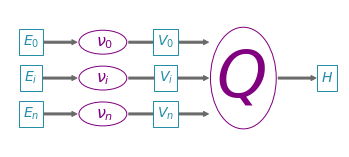
\includegraphics[width=1\textwidth]{../paper/figures/path_of_q.png}
    \end{figure}
\end{frame}


\subsection{Measurable Visual Components $M$}

\begin{frame}<presentation:1|handout:0>{Measurable Visual Components}
    \begin{columns}
        \column{0.31\textwidth}
        \begin{equation*}
            \begin{tikzcd}[ampersand replacement=\&, row sep=huge]
                \onslide*<1|handout:1>{\vfiberc}
                \onslide*<1|handout:1>{\arrow[r, hook]} \& 
                \onslide*<1|handout:1>{\vtotalc} 
                \onslide*<1|handout:1>{\arrow[d, "\pi"']} \\
                \& 
                \onslide*<1|handout:1>{\dbasec} 
                \onslide*<1|handout:1>{\arrow[u, "\vsectionc \in \cgamma{\opensetc}{\vtotalc\restriction_{\opensetc}}"', bend right, pos=.5]}
            \end{tikzcd}
        \end{equation*}
        \column{0.69\textwidth}
    \only<1|handout:1>{
        \begin{description}[style=nextline]
            \item[\textcolor{total}{Data \vtotalc}]{continuity + visual fields}
            \item[\textcolor{base}{Continuity \dbasec}]{data continuity}
            \item[\textcolor{fiber}{components \vfiberc}] {visual components \cite{bertinIIPropertiesGraphic2011} of a graphic, e.g. x and y position, area, color, line thickness}
        \end{description}
        }
    \end{columns}
    \pause 
    \only<1|handout:1>{
        \begin{alertblock}{}
            \begin{description}[style=nextline]
                \item[\textcolor{section}{visual components}]{$\cgamma{\opensetc}{\vtotalc\restriction_{\opensetc}} \coloneqq \big\{\vsectionc: \opensetc\rightarrow \vtotalc\restriction_{\opensetc} \; \bigm{\vert} \pi(\vsectionc(\dbasepointc)) = \dbasepointc\;for\, all\; \dbasepointc \in \opensetc \big\}$}
            \end{description}
        \end{alertblock}
    }
\end{frame}

\begin{frame}<presentation:1|handout:0>
    \frametitle{Data to Visual Transformation: $\vchannelc: \dfiberc_{\dbasepointc} \mapsto \vfiberc_{\dbasepointc}$}
    \begin{columns}
    \column{.5\textwidth}
    \begin{equation*}
        \begin{tikzcd}[ampersand replacement=\&]
        \dtotalc 
        \arrow[rr, "\vchannelc_{\dbasec}", color=artist] 
        \arrow[rd, "\pi" description, dotted] 
        \arrow[ddd, "\dfuncc_{\dtotalc}"', color=action] 
        \& \& 
        \vtotalc 
        \arrow[ld, "\pi" description, dotted] 
        \arrow[ddd, "\dfuncc_{\vtotalc}", color=action] \\
        \& \dbasec \&  \\
        \& \dbasec^{\prime} 
        \arrow[u, "\dfunchc" description, color=action] \& \\
        \dfuncpullc\dtotalc 
        \arrow[ru, "\pi" description, dotted] 
        \arrow[rr, "\vchannel_{\dbasec}"', color=artist] 
        \& \& 
        \dfuncpullc\dtotalc 
        \arrow[lu, "\pi" description, dotted]
        \end{tikzcd}
    \end{equation*}
    \column{.5\textwidth} 
    \begin{equation}
    \begin{tikzcd}[ampersand replacement=\&, row sep=huge]
        \dfiberc_{\dbasepointc} 
        \arrow[rr, "\vchannelc_{\dtotalc} ", maps to, color=artist] 
        \arrow[rrdd, "{\vchannelc_{\dtotalc,\vtotalc}}" description, dashed, maps to, color=artist] 
        \&  \& 
        \vfiberc_{\dbasepointc}\coloneqq {\dfiberc_{\dbasepointc}}^{\vtotalc} \arrow[dd, "\vchannelc_{\vtotalc}", maps to, color=artist] \\
        \& \& \\
        \&  \& {\vfiberc_{\dbasepointc}}^{\vtotalc}
        \end{tikzcd}
    \end{equation}
    \end{columns}
    % fix corner to be V 
    % fix \phi to be \phi 
    \begin{alertblock}{equivariance} 
       $\vchannelc: \dfuncc_{\dtotalc} \rightarrow \dfuncc_{\vtotalc}$ is a functor such that 
       \begin{description}
           \item[equivariance] {$\vchannelc(\dfuncc(\dsectionc(\dfunchc_{\dtotalc}^{-1}(\dbasepointc)))) = \dfuncc_{\vtotalc}(\vchannelc(\dsectionc(\dfunchc_{\vtotalc}^{-1}(\dbasepointc))))$\\$\dfunchc_{\dtotalc}(\dbasepointc^{\prime}) = \dfunchc_{\vtotalc}(\dbasepointc^{\prime})$}
           \item[continuity] $\lim\limits_{x\to \dbasepointc}(\vchannelc(\dsectionc(x))) = \vchannelc(\dsectionc(\dbasepointc))$ for all $\dbasepointc \in \dbasec$ 
       \end{description}
\end{alertblock}
\end{frame}  


\begin{frame}<presentation:1|handout:0>\frametitle{$\vchannelc:\dfuncc_{\dtotalc} \rightarrow \dfuncc_{\vtotalc}$: Stevens' Scales \cite{stevensTheoryScalesMeasurement1946}}
    \begin{table}[H]
        \begin{tabularx}{\textwidth}{|l|l|X|}\toprule
            \textbf{scale} & \textbf{group} & \textbf{constraint} \\\midrule
            nominal & permutation &  $\text{if } \delement_1 \neq \delement_2 \text{ then } \vchannel (\delement_1) \neq\vchannel(\delement_2)$\\
            ordinal &  monotonic & $\text{if } \delement_1 \leq \delement_2 \text{ then } \vchannel (\delement_1) \leq \vchannel(\delement_2)$\\
            interval &  translation &  $\vchannel (\delement + c) = \vchannel(\delement) + \vchannel(c)$ \\
            ratio &  scaling &  $\vchannel(\delement* c) = \vchannel(\delement)*\vchannel(c) $\\ \bottomrule
        \end{tabularx}
    \end{table}
\end{frame}


\begin{frame}<presentation:1|handout:0>
    \frametitle{Shared Components: $\vchannelc = \prod\limits_{i=0}^{n}\vchannelc_i$}
    \begin{equation}
        \begin{tikzcd}[ampersand replacement=\&]
            \dfiberc_a\times \dfiberc_b 
            \arrow[rr, "\vchannelc", color=artist, maps to] 
            \arrow[rd, "p_{\dfiberc}", color=fiber] \& \& \vfiberc_a\times \vfiberc_b 
            \arrow[rd, "p_{\vfiberc}", color=fiber] \& \\    \& 
            \dfiberc_{a} 
            \arrow[rr, "\vchannelc_{a}", dashed, maps to, color=artist] \& \& \vfiberc_a \\
            \dfiberc_a\times \dfiberc_c 
            \arrow[rr, "\vchannelc^{\prime}", color=artist, maps to] 
            \arrow[ru, "p_{\dfiberc^{\prime}}"', color=fiber] \& \& 
            {\vfiberc_a}^{\prime}\times {\vfiberc_c}^{\prime} 
            \arrow[ru, "p_{\vfiberc^{\prime}}"', color=fiber] \&           
            \end{tikzcd}
    \end{equation}
    \begin{alertblock}{Consistent Transformations \cite{hullmanKeeping2018}}
        if $p_{\dfiberc} = p_{\dfiberc^{\prime}}$ then $p_{\vfiberc}(\vchannelc(\dsectionc)) = p_{\vfiberc^{\prime}}(\vchannelc^{\prime}(\dsectionc^{\prime}))$ s.t. there exists a transformation $\vchannelc_a: \dfiberc_{a}\rightarrow \vfiberc_{a}$
    \end{alertblock}
\end{frame}


\subsection{Combining Components into Visualizations}

\begin{frame}<presentation:1|handout:0>{Assembly Function $\vmarkc$}
    \begin{equation*}
        \begin{tikzcd}[ampersand replacement = \&]
            \cgamma{\opensetc}{\vtotalc\restriction_{\opensetc}} 
            \arrow[rrrr, "\vmarkc", Rightarrow, color=artist] 
            \arrow[ddd, "\dfuncc_{\vtotalc}"', color=action] 
            \& \& \& \& 
            \cgamma{\opensetgc}{\gtotalc\restriction_{\opensetgc}} 
            \arrow[ddd, "\dfuncc_{\gtotalc}", color=action]  \\
            \& 
            \opensetc 
            \arrow[lu, maps to, color=sheaf] 
             \&  \& 
            \opensetgc 
            \arrow[ll, "\vindexc"', color=functor] 
            \arrow[ru, maps to, color=sheaf]  \& \\
            \& 
            \opensetc^{\prime} 
            \arrow[u, "\dfunchc_{\dtotalc}", color=action] 
            \arrow[ld, maps to, color=sheaf] 
            \&  \& 
            \opensetgc^{\prime} 
            \arrow[ll, "\vindexc"', color=functor] 
            \arrow[u, "\dfunchc_{\gtotalc}"', color=action] 
            \arrow[rd, maps to, color=functor] \& \\
            \cgamma{\opensetc^{\prime}}{\dfuncpullc_{\vtotalc}\vtotalc\restriction_{\opensetc^{\prime}}}
            \arrow[rrrr, "\vmarkc", Rightarrow, color=artist] 
            \& \&  \& \& 
            \cgamma{\opensetgc^{\prime}}{\dfuncpullc_{\gtotalc}\gtotalc\restriction_{\opensetgc^{\prime}}}
            \end{tikzcd}
        \end{equation*}
    \begin{alertblock}{equivariance}
       \begin{equation*}
        \vmarkc(\dfuncc_{\vtotalc}(\vsectionc(\dfunchc_{\vtotalc}^{-1}(\dbasepointc^{\prime})))) = \dfuncc_{\gtotalc}(\vmarkc((\vsectionc(\dfunchc_{\gtotalc}^{-1}(\vindexprec(\dbasepointc^{\prime}))))))
       \end{equation*}
    \end{alertblock}
\end{frame}

\begin{frame}<presentation:1|handout:0>{Implementation Choices: $\vartistc_{\opensetc} = \vartistc_{\opensetgc}$}
    \begin{equation*}
    \begin{tikzcd}[ampersand replacement = \&, column sep=small]
        \cgamma{\opensetgc}{\vindexpullc\dtotalc\restriction_{\opensetgc}}  
        \arrow[r, "\vchannelc", maps to, color=artist] 
        \arrow[rrrr, "\vartistc_{\opensetgc}", Rightarrow, bend left, color=artist] \& 
        \cgamma{\opensetgc}{\vindexpullc\vtotalc\restriction_{\opensetgc}} \& 
        \cgamma{\opensetgc}{\vindexpullc\vtotalc\restriction_{\opensetgc}}  
        \arrow[rr, "\vmarkc^*", no head, Rightarrow, color=artist] \&  \& 
        \cgamma{\opensetgc}{\gtotalc\restriction_{\opensetgc}}  
        \arrow[dd, "\vindexpushc", color=functor] \\
        \& \& \& \& \\
        \cgamma{\opensetc}{\dtotalc\restriction_{\opensetc}}  
        \arrow[uu, "\vindexpullc", color=functor] 
        \arrow[r, "\vchannelc", maps to, color=artist] 
        \arrow[rrrr, "\vartistc_{\opensetc}", Rightarrow, bend right, color=artist] 
        \& 
        \cgamma{\opensetc}{\vtotalc\restriction_{\opensetc}}  
        \arrow[uu, "\vindexpullc"', color=functor] \& 
        \cgamma{\opensetc}{\vtotalc\restriction_{\opensetc}}
        \arrow[rr, "\vmarkc_*", Rightarrow, color=artist] 
        \arrow[uu, "\vindexpullc", color=functor] 
        \arrow[rruu, "\vmarkc", Rightarrow, color=artist] 
        \&  \& 
        \cgamma{\opensetgc}{\vindexpushc\gtotalc\restriction_{\opensetc}}
    \end{tikzcd}
    \end{equation*}
\end{frame}

\begin{frame}<presentation:1|handout:0>{Components to Graphic}
    \begin{figure}
        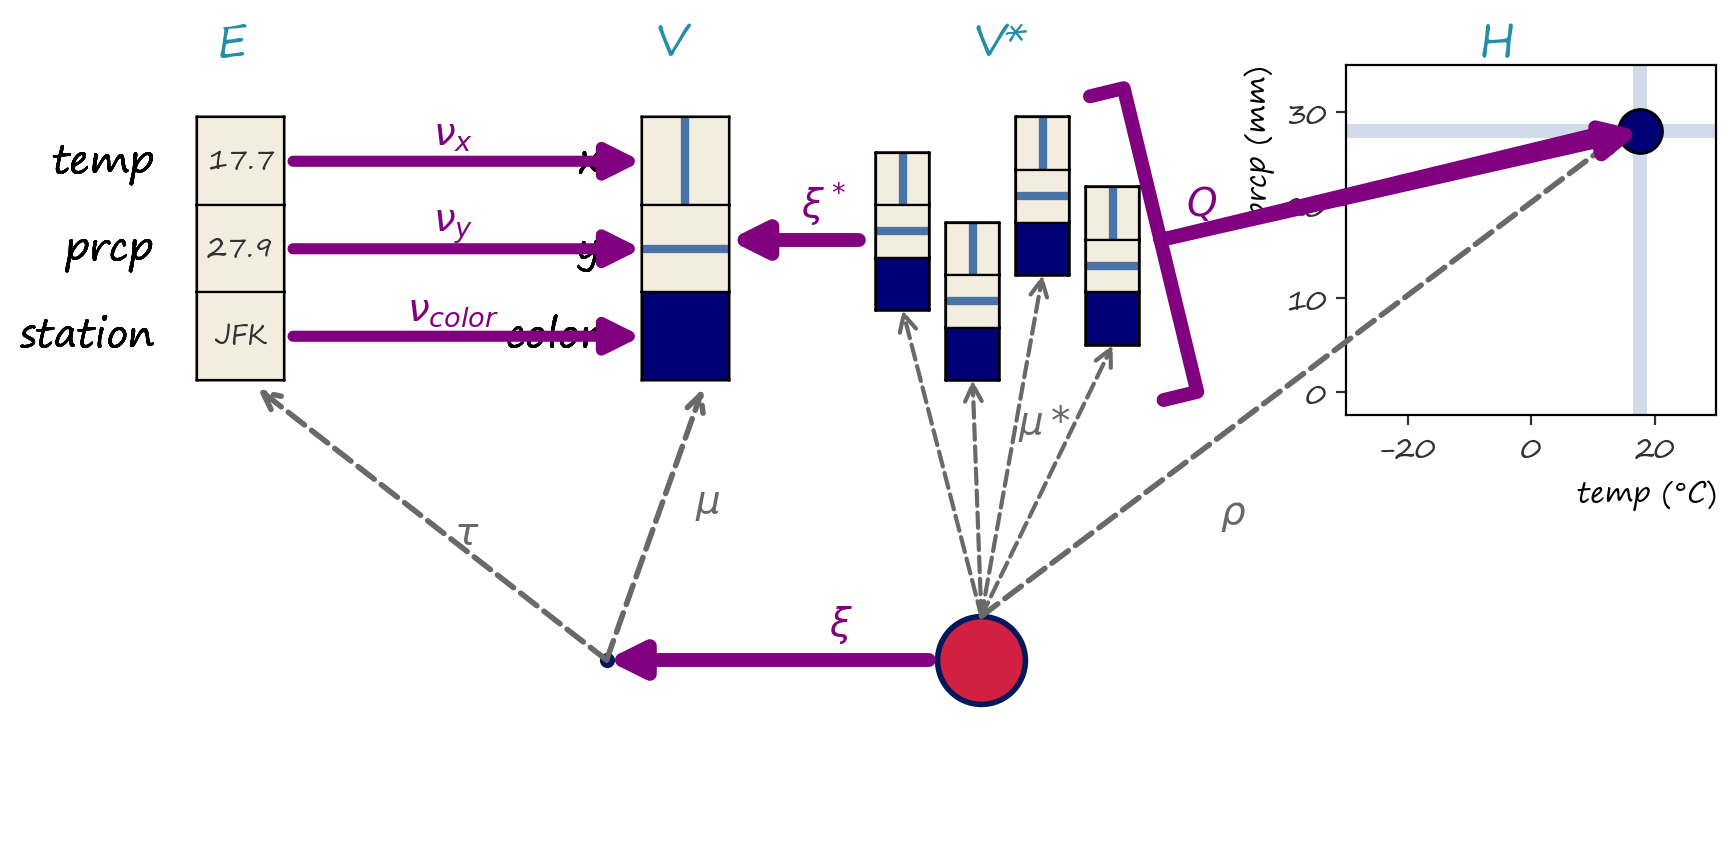
\includegraphics[scale=.15]{../paper/figures/qhat.png}
    \end{figure}
\end{frame}
\end{document}